    %------------------------------------------------------------------------------
% CV in Latex
% Author : Charles Rambo
% Based off of: https://github.com/sb2nov/resume and Jake's Resume on Overleaf
% Most recently updated version may be found at https://github.com/fizixmastr 
% License : MIT
%------------------------------------------------------------------------------

\documentclass[A4,11pt]{article}
\usepackage[a4paper, top=1.0cm, bottom=1.0cm, left=1.3cm, right=1.3cm]{geometry}
%\documentclass[letterpaper,11pt]{article} %For use in US
\usepackage{latexsym}
% \usepackage[empty]{fullpage}
\usepackage{titlesec}
\usepackage{marvosym}
\usepackage[usenames,dvipsnames]{color}
\usepackage{verbatim}
\usepackage{enumitem}
\setlist[itemize]{itemsep=2pt, topsep=2pt}
\usepackage[hidelinks]{hyperref}
\usepackage[english]{babel}
\usepackage{tabularx}
\usepackage{tikz}
\input{glyphtounicode}

\usepackage{fontawesome}
\input{glyphtounicode}

\definecolor{navy}{RGB}{78, 81, 128}
\begin{comment}
I am by no means a professional when it comes to the CV's/resumes, I have
received various trainings on how to write a CV and resume from my high 
school, as well as the Austin College and University of Eastern Finland's
career counseling departments. As I intend to share my CV as a template, I 
feel that it is my responsibility to provide explanations of my work.
\end{comment}


%-----FONT OPTIONS-------------------------------------------------------------
\begin{comment}
The font of the document will impact not just how readable it is, but how it is
perceived. In the "The Craft of Scientific Writing" by Michael Alley, shares a
common fonts for publication as well as their use. I have chosen to use
Palatino for its legibility, some others are given below. There is far too much
about typography to discus here. Note: serif fonts have short projecting
strokes, sans-serif fonts are sans (without) these strokes.
\end{comment}


% serif
 \usepackage{palatino}
% \usepackage{times} %This is the default as well
% \usepackage{charter}

% sans-serif
% \usepackage{helvet}
% \usepackage[sfdefault]{noto-sans}
% \usepackage[default]{sourcesanspro}

%-----PAGE SETUP---------------------------------------------------------------

% % Adjust margins
% \addtolength{\oddsidemargin}{-1cm}
% \addtolength{\evensidemargin}{-1cm}
% \addtolength{\textwidth}{2cm}
% \addtolength{\topmargin}{-1cm}
% \addtolength{\textheight}{2cm}

% Margins for US Letter size
%\addtolength{\oddsidemargin}{-0.5in}
%\addtolength{\evensidemargin}{-0.5in}
%\addtolength{\textwidth}{1in}
%\addtolength{\topmargin}{-.5in}
%\addtolength{\textheight}{1.0in}

\urlstyle{same}

\raggedbottom
\raggedright
\setlength{\tabcolsep}{0cm}

% Sections formatting
\titleformat{\section}{
  \vspace{-4pt}\scshape\raggedright\large
}{}{0em}{}[\color{black}\titlerule \vspace{-5pt}]

% Ensure that .pdf is machine readable/ATS parsable
\pdfgentounicode=1

%-----CUSTOM COMMANDS FOR FORMATTING SECTIONS----------------------------------
\newcommand{\CVItem}[1]{
  \item\small{
    {#1 \vspace{-2pt}}
  }
}

\newcommand{\CVSubheading}[4]{
  \vspace{-2pt}\item
    \begin{tabular*}{0.97\textwidth}[t]{l@{\extracolsep{\fill}}r}
      \textbf{#1} & #2 \\
      \small#3 & \small #4 \\
    \end{tabular*}\vspace{-7pt}
}

\newcommand{\CVSubSubheading}[2]{
    \item
    \begin{tabular*}{0.97\textwidth}{l@{\extracolsep{\fill}}r}
      \text{\small#1} & \text{\small #2} \\
    \end{tabular*}\vspace{-7pt}
}

\newcommand{\CVSubItem}[1]{\CVItem{#1}\vspace{-4pt}}

\renewcommand\labelitemii{$\vcenter{\hbox{\tiny$\bullet$}}$}

\newcommand{\CVSubHeadingListStart}{\begin{itemize}[leftmargin=0.5cm, label={}]}
% \newcommand{\resumeSubHeadingListStart}{\begin{itemize}[leftmargin=0.15in, label={}]} % Uncomment for US
\newcommand{\CVSubHeadingListEnd}{\end{itemize}}
\newcommand{\CVItemListStart}{\begin{itemize}}
\newcommand{\CVItemListEnd}{\end{itemize}\vspace{-5pt}}

%------------------------------------------------------------------------------
% CV STARTS HERE  %
%------------------------------------------------------------------------------
\begin{document}
\pagenumbering{gobble}
%-----HEADING------------------------------------------------------------------
\begin{comment}
In Europe it is common to include a picture of ones self in the CV. Select
which heading appropriate for the document you are creating.
\end{comment}


% --- Left Side: Contact Information ---
\begin{minipage}[c]{0.7\textwidth}
    {\huge \scshape \color{navy} Fatemeh (Negin) Tavakkoli} \\ \vspace{4pt}
    {\large Data Scientist | Computational Researcher} \\ \vspace{2pt}
    \rule{\linewidth}{0.4pt} \\ \vspace{3pt}
    
    \small
    \begin{tabular}{ll @{\hspace{20pt}} ll}
        \faMapMarker \hspace{6pt} & Sodener Str. 11, 14197 Berlin & \faEnvelope \hspace{6pt} & \href{mailto:tavakkolin.1991@gmail.com}{tavakkolin.1991@gmail.com} \\ \vspace{4pt}
        \faPhone     & +49 (176) 32259016 & \faLink & \href{https://github.com/negintavakkoli}{\faGithub} \hspace{4pt} \href{https://gitlab.mpcdf.mpg.de/ftava}{\faGitlab} \hspace{4pt} \href{https://www.linkedin.com/in/negin-tavakkoli/}{\faLinkedin}
    \end{tabular}
\end{minipage}%
\hfill
% --- Right Side: Profile Picture ---
\begin{minipage}{0.30\textwidth}
\begin{flushright}
    % \flushright % Aligns the picture to the far right edge
    \begin{tikzpicture}
        % The circle is 4cm wide (radius 2cm)
        \clip (0,0) circle (2cm); 
        
        % The image must be AT LEAST 4cm wide to cover the circle
        % Adjust the 'at (0,0)' if you need to shift your face to the center
        \node at (0,0) {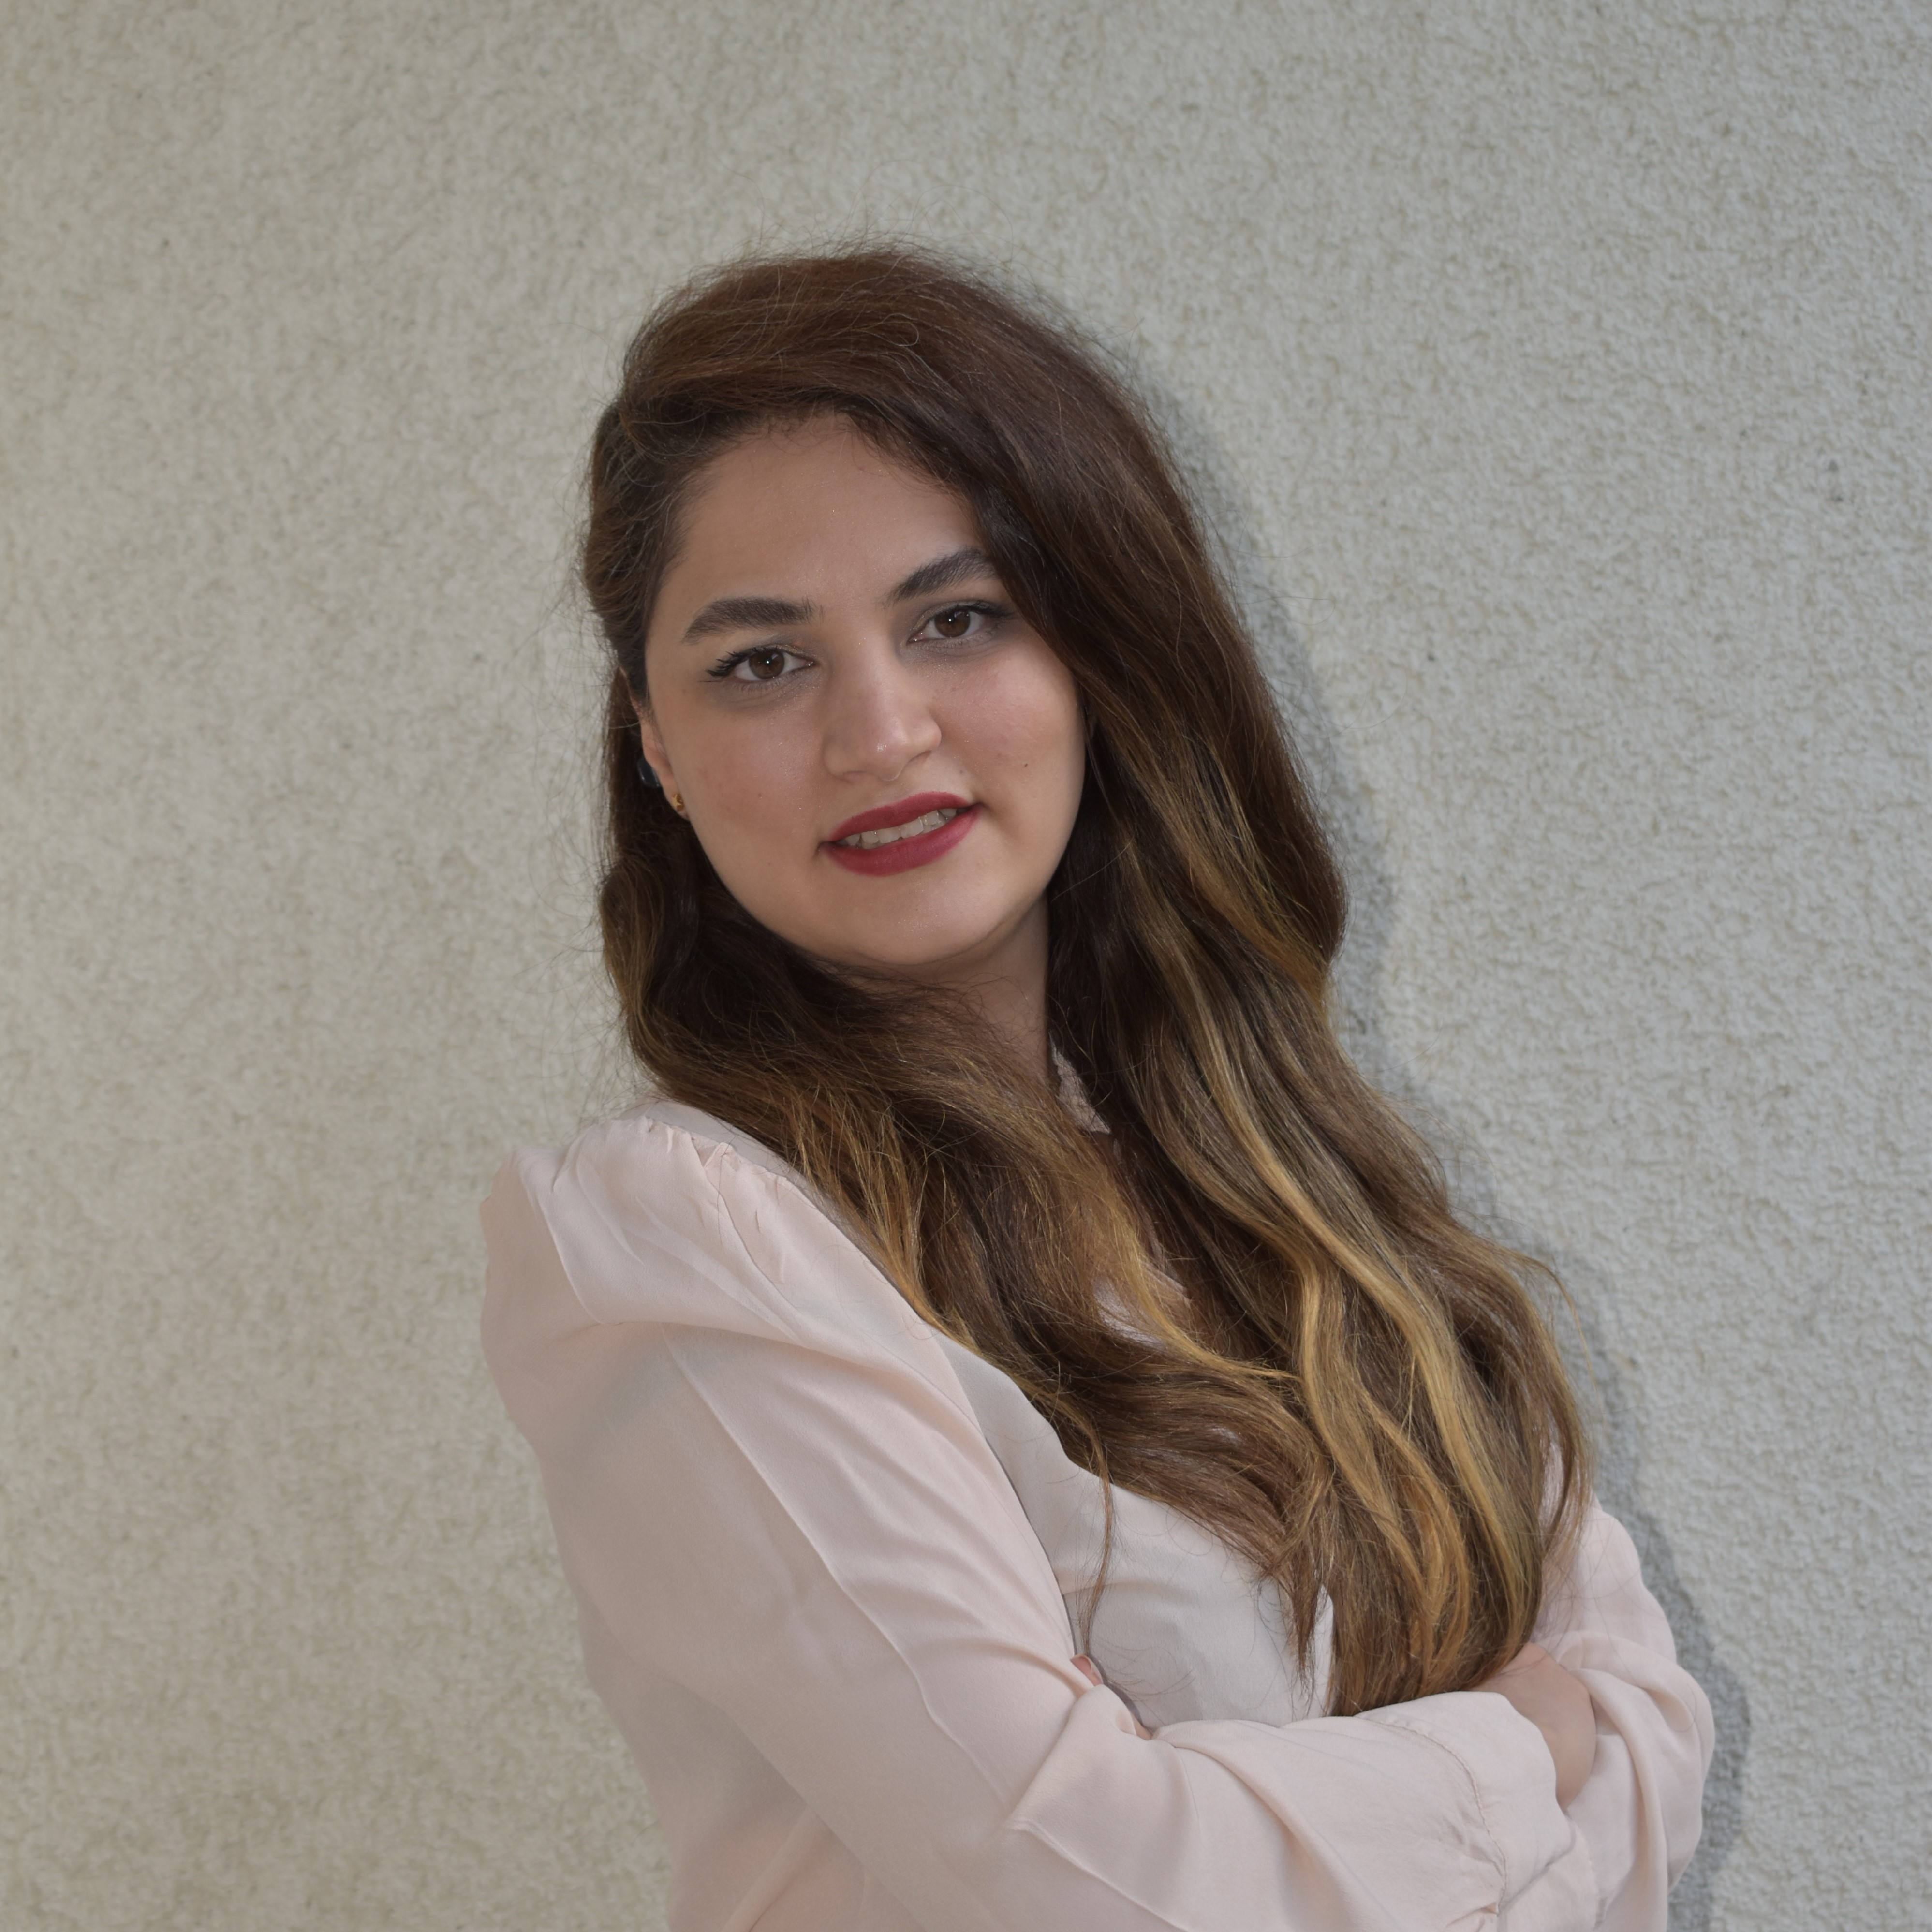
\includegraphics[width=4.5cm]{Negin_Sqar_Big.jpg}}; 
    \end{tikzpicture}
    \end{flushright}
\end{minipage}




\begin{comment}
This CV was written for specifically for positions I was applying for in
academia, and then modified to be a template.

A standard CV is about two pages long where as a resume in the US is one page.
sections can be added and removed here with this in mind. In my experience, 
education, and applicable work experience and skills are the most import things
to include on a resume. For a CV the Europass CV suggests the categories: Work
Experience, Education and Training, Language Skills, Digital Skills,
Communication and Interpersonal Skills, Conferences and Seminars, Creative Works
Driver's License, Hobbies and Interests, Honors and Awards, Management and
Leadership Skills, Networks and Memberships, Organizational Skills, Projects,
Publications, Recommendations, Social and Political Activities, Volunteering.

Your goal is to convey a who, what , when, where, why for every item you share. 
The who is obviously you, but I believe the rest should be done in that order.
For example below. An employer cares most about the degree held and typically 
less about the institution or where it is located (This is still good 
information though). Whatever order you choose be consistent throughout.
\end{comment}




\section*{Profile}
\begin{itemize}
    \item AI Engineer specializing in the sustainable implementation of LLMs and Trusted Learning Analytics within university infrastructures. Expert in high-performance simulation and mathematical optimization, with a proven track record of architecting scalable, data-compliant AI pilot scenarios for higher education administration and teaching.
    

    % \item Proficient in \textbf{Python, PyTorch, and high-performance C++}
\end{itemize}

%-----EDUCATION----------------------------------------------------------------
% \section{Education}
%   \CVSubHeadingListStart
  
%   %    \CVSubheading % Example
% %      {Degree Achieved}{Years of Study}
% %      {Institution of Study}{Where it is located}
 
%     \CVSubheading
%       {{{\href{https://www.fu-berlin.de/en/index.html}{\color{navy} Freie Universität Berlin}} \emph{\small{}}}}{Oct.2021 - Now}
%       {M.Sc. Computational Science, Advisor: Dr. Sebastian Matera }{Berlin, Germany}
%               \CVItemListStart
%         \CVItem{Expected graduation: November 2025}
%     \CVItemListEnd


     
% %    \CVSubheading % Example
% %      {Degree Achieved}{Years of Study}
% %      {Institution of Study}{Where it is located}
 
%     \CVSubheading
%       {{{\href{http://shdu.ac.ir/en/home}{\color{navy} Shehab-e Danesh University}} \emph{\small{}}}}{Sep.2010 - Oct.2015}
%       {B.Sc. Computer Engineering, Advisor: Dr. Ali Sohofi}{Qom, Iran} \\ 
%     %     \CVItemListStart
%     %     \CVItem{Thesis: developing a knowledge-based system, a platform for creating, browsing, and searching data}
%     % \CVItemListEnd

%   \CVSubHeadingListEnd



    
% %------------------------------------------------------------------------------





% % This part is appropriate for Applied math
% % \section{Selected Profession and Researches}
% %   \CVSubHeadingListStart
% % %    \CVSubheading
% % %      {Title of Work}{When it was done}
% % %      {Institution you worked with}{unused}
% % % This part is appropriate for Applied math
% % \CVSubheading
% %       {{Fritz Haber Institute of the Max Planck Society| Internship}}{Berlin, Germany}
% %       {Kinetic Monte Carlo Simulation for Prey-Predator Equation,$|$ \emph{\small{Python C++}}}{}
% %       \CVItemListStart
% %         % \CVItem{Automated Essay Grading }
% %       \CVItem{Modeling predator and Ising modeling }
      
% %         % \CVItem{Automated Short Answer Grading (ASAG)}
        
% %       \CVItemListEnd

% % % This part is appropriate for Applied math
% % \CVSubheading
% %       {{Weierstrass Institute Berlin}}{2023}
% %       {Modeling Heat Circulation in a 2D Room,$|$ \emph{\small{Python FEniCS}}}{Berlin, Germany}
% %       \CVItemListStart
% %         % \CVItem{Automated Essay Grading }
% %       \CVItem{Modeling heat circulation using weak formulation }
      
% %         % \CVItem{Automated Short Answer Grading (ASAG)}
        
% %       \CVItemListEnd


% % % This part is appropriate for ComSci
% % \CVSubheading
% %       {{AI for summative assessment and feedback,$|$ \emph{\small{Python, BERT}}}}{2023}
% %       {Freie Universität Berlin/ IMPACT project}{Berlin, Germany}
% %       \CVItemListStart
% %         \CVItem{Automated Essay Grading }
% %       \CVItem{Using Deep Learning Model for Natural language Processing }
      
% %         \CVItem{Automated Short Answer Grading (ASAG)}
        
% %       \CVItemListEnd


% % % This part is appropriate for Applied math
% % \CVSubheading
% %       {{Gravitational N-Body Simulation,$|$ \emph{\small{Python}}}}{2023}
% %       {Freie Universität Berlin/ Mathematic Department}{Berlin, Germany}
% %       \CVItemListStart
% %       \CVItem{Simulation of interaction of a N-Body System based on their gravity}
% %         \CVItem{Using the NASA's dataset }
        
% %       \CVItemListEnd

% % % This part is appropriate for Applied CompSci
% % % \CVSubheading
% % %       {{Reanalysis Parameters for Lightning Frequency,$|$ \emph{\small{Python}}}}{2023}
% % %       {Freie Universität Berlin/ Meteorological  Department}{Berlin, Germany}
% % %       \CVItemListStart
% % %       \CVItem{Combining Observation dataset with reanalysis lightning dataset}
% % %         \CVItem{Compared 2-dimention parameters }
        
% % %       \CVItemListEnd

% % % This part is appropriate for ComSci
% % \CVSubheading
% %       {{Deforestation Detection,$|$ \emph{\small{R, QGIS}}}}{2022}
% %       {Freie Universität Berlin}{Berlin, Germany}
% %       \CVItemListStart
% %       \CVItem{Classification Land Cover Area in the West-Coast of Australia with Multi-Spectral Satellite Data}
% %         \CVItem{Change Detection Using Classification-Based Detection and Vegetation Indices }
        
% %       \CVItemListEnd



% % % This part is appropriate for ComSci
% %      \CVSubheading
% %       {{Zoodpaz, a Persian Ingredient Corpus$|$ \emph{\small{Python, Django}}}}{2021}
% %       {Freelance}{}
% %       \CVItemListStart
% %       \CVItem{A Corpus of Ingredients, Attained From Recipes by Doccano}
% %         \CVItem{Enable to Extract Ingredient From Others Recipes}
        
% %       \CVItemListEnd
        
% %       % \CVSubheading
% %       % {{Maglet, a Persian journal recommender system $|$ \emph{\small{Python, Django}}}}{2020}
% %       % {Freelance}{}
% %       % \CVItemListStart
      
% %       %   \CVItem{Maglet, a recommendation journal system for manuscripts, based on their abstracts}
% %       %   \CVItem{Using text similarity measures and Lucence indexing to 
% %       %   find the most related journals}
% %       % \CVItemListEnd
      
% %       % \CVSubheading
% %       % {{Hamsoo24, a knowledge manager modular enterprise social network (ESN)}}{2016 - 2019}
% %       % {{\href{https://www.sepehrmahan.com/}{\color{navy} Sepehr Mahan}}}{Tehran, Iran}
% %       %       \CVItemListStart
% %       %   \CVItem{A collaborative software, making Team's communication easier}
% %       %   \CVItem{Using different integrated modules to unify employees' desk}
% %       % \CVItemListEnd
      
% %       %    \CVSubheading
% %       % {{Thesis: Public Article $|$ \emph{\small{ASP.NET, SQL Server}}}}{2014}
% %       % {{\href{http://shdu.ac.ir/en/home}{\color{navy} Shehab-e Danesh University}}}{Qom, Iran}
% %       %   \CVItemListStart
% %       %   \CVItem{A Searchable Platform for Creating and Browsing Information}
% %       % \CVItemListEnd
      
% %      % \CVSubheading
% %      %  {{Professor Assistant Project $|$ \emph{\small{Java}}}}{2013}
% %      %  {{\href{http://shdu.ac.ir/en/home}{\color{navy} Shehab-e Danesh University}}}{Qom, Iran}
% %      %        \CVItemListStart
% %      %    \CVItem{An Assistant System For Professors to Manage Their Classes, Students, and Documents }
% %      %  \CVItemListEnd
% %   \CVSubHeadingListEnd





\section{WORK EXPERIENCE}
\CVSubHeadingListStart






\CVSubheading
    {Data Scientist @ \href{https://impact.studiumdigitale.uni-frankfurt.de}{IMPACT Project}}
    {\textit{Freie Universität Berlin}}
    {Berlin, Germany}
    {08.2022 -- 11.2025}

    % {Berlin, Germany}
    
 

    \CVItemListStart
   \CVItem{\textbf{Project Scope:} Implementation of AI-based feedback and assessment with Trusted Learning Analytics in Higher Education Institutions (HEIs).}
   
     \CVItem{Architected a web-based AI assistant for summative assessment, utilizing LLMs to provide (semi-) automated evaluation of complex student responses.}
     
            \CVItem{Designed, fine-tuned, and deployed neural models (BERT/LLaMA) using PyTorch for scalable evaluation tasks}
            % \CVItem{Designed preprocessing and embedding pipelines (subword tokenization, padding, batching)}
        

           \CVItem{Developed GPU-accelerated infrastructure for model inference using Docker + Linux servers}
        % \CVItem{Designed and implemented infrastructure solutions for efficient and reproducible AI model deployment at scale.}

        \CVItem{Design and implement infrastructure solutions for efficient, reproducible AI model deployment at scale, including deploying a LLaMA model on a GPU server with full management of containerization, dependencies, model weights, quantization options, and API endpoints for downstream NLP and NLG tasks.}
    \CVItemListEnd





\CVSubheading
  {Research Internship @ Multiscale Modeling Group}
  {\textit{Fritz Haber Institute of the Max Planck Society}}
  {Berlin, Germany}
  {10.2024 -- 03.2026}

% \textit{Research Title:} Simulation of Lotka–Volterra Dynamics Using Markove Jump Processing Method

\CVItemListStart
 % \CVItem{Employmented a scalable \textit{kinetic Monte Carlo (kMC)} framework for compartment-based spatiotemporal master equations}
    \CVItem{Designed and implemented a high-performance Python–C++ interface.}
    \CVItem{Scaled stochastic simulation frameworks across AWS ParallelCluster environments to handle high-dimensional master equations.}
    \CVItem{Optimized algorithmic performance to reduce execution time, ensuring scalable and sustainable implementation within high-dimensional computing environments.}
    
    
    
\CVItemListEnd




    
    \CVSubheading
    {Researcher and Developer}
    {\textit{Sepehr Mahan}}
    {Tehran, Iran}
    {07.2016 -- 03.2021}
    
    \CVItemListStart
        \CVItem{Applied supervised machine learning methods to develop customer segmentation models for data-driven decision making.}
        \CVItem{Led agile development processes in a Scrum-master role, overseeing Git workflows and coordinating team efforts to ensure high code quality, reproducibility, and efficient collaboration.}
    \CVItemListEnd
    % \CVSubheading
    %   {Support Expert}{July 2016 - April 2018}
    %   {{\href{https://www.sepehrmahan.com/}{\color{navy} Sepehr Mahan}}}{Tehran, Iran}
    %   \CVItemListStart
    %     % \CVItem{Analysing systems and designing use cases, forms, databases}
    %          \CVItem{Deployment systems based on the requirements of customers}
    %     \CVItem{Providing test planning for manual test}
    
% %------------------------------------------------------------------------------



% \section{SELECTED RESEARCH EXPERIENCE}

% \CVSubHeadingListStart

% \CVSubheading
%   {Research Internship @ Multiscale Modeling Group}
%   {{Fritz Haber Institute of the Max Planck Society}}
%   {Berlin, Germany}
%   {10.2024 -- 03.2025}

% \textit{Research Title:} Simulation of Lotka–Volterra Dynamics Using Markove Jump Processing Method

% \CVItemListStart
% \CVItem{Employment agent-based and stochastic simulation frameworks for modeling complex dynamical systems, specifically the Lotka–Volterra equations, in both on-lattice and off-lattice environments.}
% \CVItem{Wrote scalable and portable code capable of efficiently handling varying lattice sizes.}
% \CVItem{Implemented a stochastic Lotka–Volterra model to analyze predator–prey population dynamics driven by rate of birth and death processes.}
% \CVItemListEnd

% \CVSubheading %Example
%       {Seminar Research Project}{Freie Universität Berlin}
%       {Berlin, Germany}{12/2022 – 02/2023}
      
%         {\underline{Research Title:} Climate variable modeling using the Planet Simulator (PLASIM)}
%         \CVItemListStart
%         \CVItem{Processed large-scale geospatial datasets (ERA5) using cloud-based and high-performance computing environments}
%         \CVItem{Applied advanced spatial analysis and scientific visualization techniques to evaluate environmental dynamics, supporting geospatial research that aligns with modern sensing and mapping technologies.}
%         \CVItem{Simulated 100-year vegetation responses under five atmospheric $CO_2$ scenarios using PlaSim, analyzing key indicators such as Leaf Area Index (LAI) and Water-Limited Gross Primary Production (WLGPP).}
%         \CVItem{Compared vegetation dynamics in the Amazon Rainforest and Sahara Desert, finding strong $CO_2$-driven increases in water-use efficiency in the Amazon but minimal change in the Sahara.}
%         \CVItemListEnd
%         \CVItem{Applied HPC numerical methods in mixed Taylor–Hood function spaces for multiphysics simulations.}
%         \CVItem{Mixed Taylor-Hood function space (velocity, pressure, temperature)}
%            \CVItem{A Member of Research Impact Team}
%       \CVItemListEnd

%     \CVSubheading %Example
%       {Seminar Research Project}{Weierstrass Institute}
%       {Berlin, Germany}{06.2023 - 08.2023}

%       {\underline{Research Title:} Modeling Heat Circulation in a 2D Room}
%       \CVItemListStart
%       % \CVItem{What did you do?}
%         % \CVItem{Applied HPC numerical methods in mixed Taylor–Hood function spaces for multiphysics simulations.}
%         \CVItem{Formulated a coupled incompressible Navier–Stokes and convection–diffusion model with Boussinesq approximation to describe heat circulation in a 2D room with heater and glass boundaries.}
%         \CVItem{Derived the weak formulation and implemented a mixed Taylor–Hood finite element discretization with Chorin projection to solve for velocity, pressure, and temperature fields.}
%         \CVItem{Simulated and visualized temperature, pressure, and flow fields under different heating configurations (heated circular boundary vs. heated glass) using the FEniCS Finite Element Method (FEM) software package.}
%            % \CVItem{A Member of Research Impact Team}
%       \CVItemListEnd




%     \CVSubheading %Example
%       {Seminar Research Project}{Freie Universität Berlin}
%       {Berlin, Germany}{12.2022 - 02.2023}

%       {\underline{Research Title:} Gravitational N-Body Simulation}
%       \CVItemListStart
%       % \CVItem{{What did you do?}}
%         \CVItem{Implemented a full N-body simulation engine, including data modeling and numerical integration (Position/Velocity Verlet).}
%         \CVItem{Integrated scientific datasets by generating synthetic N-body systems, importing real NASA Horizons planetary data, and modeling a Milky Way–like galaxy using the Galpy potential.}
%         \CVItem{Developed a complete simulation and visualization pipeline, including time-step integration, mechanical-energy monitoring, animation of system dynamics, and automated unit testing with CI integration.}
%       \CVItemListEnd


      
%  \CVSubheading %Example
%       {Seminar Research Project}{Freie Universität Berlin}
%       {Berlin, Germany}{12.2022 - 02.2023}

%       {\underline{Research Title:} Remote Sensing \& Land-Cover Classification – Sentinel-2 Satellite Imagery}
%       \CVItemListStart
%       % \CVItem{{What did you do?}}
%       \CVItem


%         \CVItem{Utilized GIS annotation, geospatial preprocessing, and model validation (confusion matrix)}
%       \CVItemListEnd

     % \CVSubheading
     %  {{Zoodpaz, a Persian Ingredient Corpus$|$ \emph{\small{Python, Django}}}}{2021}
     %  {Freelance}{}
     %  \CVItemListStart
     %  \CVItem{A Corpus of Ingredients, Attained From Recipes by Doccano}
     %    \CVItem{Enable to Extract Ingredient From Others Recipes}
        
     %  \CVItemListEnd
        
     %  \CVSubheading
     %  {{Maglet, a Persian journal recommender system $|$ \emph{\small{Python, Django}}}}{2020}
     %  {Freelance}{}
     %  \CVItemListStart
      
     %    \CVItem{Maglet, a recommendation journal system for manuscripts, based on their abstracts}
     %    \CVItem{Using text similarity measures and Lucence indexing to 
     %    find the most related journals}
     %  \CVItemListEnd
      


\section{Education}
  \CVSubHeadingListStart
  
  %    \CVSubheading % Example
%      {Degree Achieved}{Years of Study}
%      {Institution of Study}{Where it is located}
 
    \CVSubheading
      {{{\href{https://www.fu-berlin.de/en/index.html}{\color{navy} Freie Universität Berlin}} \emph{\small{}}}}{10.2021 - 12.2025}
      {M.Sc. Computational Science}{\textit{Thesis Advisor}: Dr. Sebastian Matera}
      
      \textbf{Thesis Title:} StochasticSimulation Algorithms for Spatiotemporal  Master Equations
      
    \CVItemListStart
   
\CVItem{Developed a Python-based interface for stochastic compartmental models, addressing the computational bottlenecks of high-dimensional master equations}
\CVItem{GPA: 1.7 }
    \CVItemListEnd


     
%    \CVSubheading % Example
%      {Degree Achieved}{Years of Study}
%      {Institution of Study}{Where it is located}
 
    \CVSubheading
      {{{\href{http://shdu.ac.ir/en/home}{\color{navy} Shehab-e Danesh University}} \emph{\small{}}}}{10.2010 - 08.2015}
      {B.Sc. Computer Engineering}{\textit{Thesis Advisor}: Dr. Ali Sohofi} 
      
      \textbf{Thesis Title:} Public Articles - A Knowledge Based System
      
      \CVItemListStart
        % \CVItem{Designed a software for collecting scientific information from users by employee UML methods.}
        % \CVItem{Design the class diagrams, Sequence diagram, and databases using DBMS.}
        \CVItem{Classified the information in terms of topic using logistic regression and TF-IDF.}
        
    \CVItemListEnd

    % \CVSubheading
      % {{{\href{http://shdu.ac.ir/en/home}{\color{navy} Allame-Majlesi High School}} \emph{\small{}}}}{09.2005 - 08.2010}
      % {Mathematical and Physics}{GPA: 14/20} 

  \CVSubHeadingListEnd



    
%------------------------------------------------------------------------------



%-----WORK EXPERIENCE------------------------------------










\section{Selected Publications}
 \begin{itemize}[leftmargin=0.5cm, label={}]
    \item {\small


     [1] \textbf{Tavakkoli, Fatemeh}, R. Ebrahimi Viand, B. Bat-Erdene, K. Reuter, S. Matera. 
    \textit{Stochastic Simulation Algorithm for Spatiotemporal Chemical Master Equations}. 
    \textbf{Poster presentation} at the DPG Spring Meeting of the Condensed Matter Section (SKM), 
    Dresden, Germany, March 2026.


    
     $[$2$]$ Mohtaj,  S. and \textbf{Fatemeh Tavakkoli}, Habibollah Asghari  \textit{PerPaDa: A Persian Paraphrase Dataset based on Implicit Crowdsourcing Data Collection}, The 2022 International Conference on Language Resources and Evaluation, \textbf{LREC 2022}, Marseille, France, June 2022\\ \vspace{4pt}}



     % $[$3$]$ Rooholamin,  M. and \textbf{Fatemeh Tavakkoli},  \textit{Added Value of Enterprise Social Networks}, Tadbir, Journal of Management, June 2019. (in Persian) \\ \vspace{4pt}
         % $[$3$]$ Mohtaj, S. and \textbf{Fatemeh Tavakkoli}, \textit{Maglet:  a Persian Journal Recommender System}, 9th International Symposium on Telecommunications (IST), Tehran, Iran, December 2018. \\ \vspace{4pt}
    %  $[$4$]$ Rooholamin, Mohsen and \textbf{Fatemeh Tavakkoli}, \textit{Hamsoo: an Enterprise Social Network}, Roshd-eFanavari: Journal of Science and Technology Park and Incubator, Tehran, Iran, under review (in Persian) \\
    % }}
 \end{itemize}






% This part is appropriate for Applied math
% \section{Selected Profession and Researches}
%   \CVSubHeadingListStart
% %    \CVSubheading
% %      {Title of Work}{When it was done}
% %      {Institution you worked with}{unused}
% % This part is appropriate for Applied math
% \CVSubheading
%       {{Fritz Haber Institute of the Max Planck Society| Internship}}{Berlin, Germany}
%       {Kinetic Monte Carlo Simulation for Prey-Predator Equation,$|$ \emph{\small{Python C++}}}{}
%       \CVItemListStart
%         % \CVItem{Automated Essay Grading }
%       \CVItem{Modeling predator and Ising modeling }
      
%         % \CVItem{Automated Short Answer Grading (ASAG)}
        
%       \CVItemListEnd

% % This part is appropriate for Applied math
% \CVSubheading
%       {{Weierstrass Institute Berlin}}{2023}
%       {Modeling Heat Circulation in a 2D Room,$|$ \emph{\small{Python FEniCS}}}{Berlin, Germany}
%       \CVItemListStart
%         % \CVItem{Automated Essay Grading }
%       \CVItem{Modeling heat circulation using weak formulation }
      
%         % \CVItem{Automated Short Answer Grading (ASAG)}
        
%       \CVItemListEnd


% % This part is appropriate for ComSci
% \CVSubheading
%       {{AI for summative assessment and feedback,$|$ \emph{\small{Python, BERT}}}}{2023}
%       {Freie Universität Berlin/ IMPACT project}{Berlin, Germany}
%       \CVItemListStart
%         \CVItem{Automated Essay Grading }
%       \CVItem{Using Deep Learning Model for Natural language Processing }
      
%         \CVItem{Automated Short Answer Grading (ASAG)}
        
%       \CVItemListEnd


% % This part is appropriate for Applied math
% \CVSubheading
%       {{Gravitational N-Body Simulation,$|$ \emph{\small{Python}}}}{2023}
%       {Freie Universität Berlin/ Mathematic Department}{Berlin, Germany}
%       \CVItemListStart
%       \CVItem{Simulation of interaction of a N-Body System based on their gravity}
%         \CVItem{Using the NASA's dataset }
        
%       \CVItemListEnd

% % This part is appropriate for Applied CompSci
% % \CVSubheading
% %       {{Reanalysis Parameters for Lightning Frequency,$|$ \emph{\small{Python}}}}{2023}
% %       {Freie Universität Berlin/ Meteorological  Department}{Berlin, Germany}
% %       \CVItemListStart
% %       \CVItem{Combining Observation dataset with reanalysis lightning dataset}
% %         \CVItem{Compared 2-dimention parameters }
        
% %       \CVItemListEnd

% % This part is appropriate for ComSci
% \CVSubheading
%       {{Deforestation Detection,$|$ \emph{\small{R, QGIS}}}}{2022}
%       {Freie Universität Berlin}{Berlin, Germany}
%       \CVItemListStart
%       \CVItem{Classification Land Cover Area in the West-Coast of Australia with Multi-Spectral Satellite Data}
%         \CVItem{Change Detection Using Classification-Based Detection and Vegetation Indices }
        
%       \CVItemListEnd



% % This part is appropriate for ComSci
%      \CVSubheading
%       {{Zoodpaz, a Persian Ingredient Corpus$|$ \emph{\small{Python, Django}}}}{2021}
%       {Freelance}{}
%       \CVItemListStart
%       \CVItem{A Corpus of Ingredients, Attained From Recipes by Doccano}
%         \CVItem{Enable to Extract Ingredient From Others Recipes}
        
%       \CVItemListEnd
        
%       % \CVSubheading
%       % {{Maglet, a Persian journal recommender system $|$ \emph{\small{Python, Django}}}}{2020}
%       % {Freelance}{}
%       % \CVItemListStart
      
%       %   \CVItem{Maglet, a recommendation journal system for manuscripts, based on their abstracts}
%       %   \CVItem{Using text similarity measures and Lucence indexing to 
%       %   find the most related journals}
%       % \CVItemListEnd
      
%       % \CVSubheading
%       % {{Hamsoo24, a knowledge manager modular enterprise social network (ESN)}}{2016 - 2019}
%       % {{\href{https://www.sepehrmahan.com/}{\color{navy} Sepehr Mahan}}}{Tehran, Iran}
%       %       \CVItemListStart
%       %   \CVItem{A collaborative software, making Team's communication easier}
%       %   \CVItem{Using different integrated modules to unify employees' desk}
%       % \CVItemListEnd
      
%       %    \CVSubheading
%       % {{Thesis: Public Article $|$ \emph{\small{ASP.NET, SQL Server}}}}{2014}
%       % {{\href{http://shdu.ac.ir/en/home}{\color{navy} Shehab-e Danesh University}}}{Qom, Iran}
%       %   \CVItemListStart
%       %   \CVItem{A Searchable Platform for Creating and Browsing Information}
%       % \CVItemListEnd
      
%      % \CVSubheading
%      %  {{Professor Assistant Project $|$ \emph{\small{Java}}}}{2013}
%      %  {{\href{http://shdu.ac.ir/en/home}{\color{navy} Shehab-e Danesh University}}}{Qom, Iran}
%      %        \CVItemListStart
%      %    \CVItem{An Assistant System For Professors to Manage Their Classes, Students, and Documents }
%      %  \CVItemListEnd
%   \CVSubHeadingListEnd

% %-----Publications-------------------------------------------------------------------


% ----------------------






% %-----PROJECTS AND RESEARCH----------------------------------------------------









% %-----PROJECTS AND RESEARCH----------------------------------------------------
% ----------- SKILLS -----------
\section{SKILLS}
 \begin{itemize}[leftmargin=0.15in, label={}]
    \small{\item{
     \textbf{Artificial Intelligence \& NLP}{: Natural Language Processing (NLP), Natural Language Generation (NLG), Transformer models (BERT, LLaMA), LLM Fine-tuning, PyTorch, Scikit-learn} \\
     
     \textbf{Scientific Computing \& Optimization}{: Python (NumPy, SciPy, Pandas), C++, Numerical Optimization, Performance-aware algorithm design, Stochastic Modeling, Uncertainty Quantification} \\
     
     \textbf{Infrastructure \& Cloud}{: AWS ParallelCluster, Microsoft Azure AI Studio (familiarity), Docker, Linux (Ubuntu/Debian), GPU-accelerated inference, HPC environments} \\
     
     \textbf{Software Engineering \& Tools}{: Git/GitHub, Reproducible Research Workflows, Streamlit, Agile/Scrum (Scrum Master experience), REST API development} \\
     
    %  \textbf{Languages}{: Persian (Native), English (Fluent: C1/B2 equivalent), German (Intermediate: B1)}
    % }}
    }}
 \end{itemize}



% ----------- SOFT SKILLS & COMPETENCIES -----------
\section{SOFT SKILLS}
 \begin{itemize}[leftmargin=0.15in, label={}]
    \small{\item{
     \textbf{Agile Project Management}{: Experienced Scrum Master coordinating cross-functional teams and Git workflows.} \\
     \textbf{Interdisciplinary Communication}{: Skilled in translating complex AI concepts for non-technical administrative and academic stakeholders.} \\
     \textbf{Analytical Problem Solving}{: Methodological and statistical competency applied to data-driven decision making.} \\
     \textbf{Risk Assessment}{: Focused on ethical perspectives and data protection in AI-based educational technologies.}
    }}
 \end{itemize}
% ----------- LANGUAGES -----------
\section{LANGUAGES}
 \begin{itemize}[leftmargin=0.15in, label={}]
    \small{\item{
     \textbf{German}{: Intermediate (B1)}  \\
     \textbf{English}{: Fluent (C1/B2 equivalent)  } \\
     \textbf{Persian}{: Native Speaker}
    }}
 \end{itemize}



% \section*{Skills}
% \begin{itemize}
%   % \setlength\itemsep{0.2em}
%   % \item \textbf{Machine Learning \& Causal Methods:} Causal inference, counterfactual reasoning, off-policy evaluation, decision-making under uncertainty
%   \item \textbf{Probabilistic Modeling:} Stochastic processes, Markov jump processes, uncertainty quantification, Robust Optimization, Monte Carlo methods
%   \item \textbf{Deep Learning:} PyTorch, transformer models (BERT, LLaMA), GPU-based training and inference
%   \item \textbf{Scientific Computing \& Systems:} Python, C++, CMake, high-performance computing (HPC), scalable simulation frameworks
%   \item \textbf{Optimization \& Numerical Methods:} Numerical optimization, event-driven simulation, performance-aware algorithm design
%   \item \textbf{Research Tools:} Linux, Git, Docker, reproducible research workflows
%   \item \textbf{Visualization \& Analysis:} Jupyter, Matplotlib
%   \item \textbf{Languages:} Persian (native), English (fluent), German (intermediate: B1)
% \end{itemize}

% % \section{SKILLS}
% % \begin{itemize}
% %     \item \textbf{Deep Learning:} PyTorch, Transformers, GPU  
% %     \item 
% %     \item \textbf{Programming:} C++, Python, CMake  
% %     \item \textbf{Simulation \& Modeling:} Stochastic Simulation, Finit Element Methods, Markov Chain
% %     % agent-based models
% %     \item \textbf{Distributed \& Cloud Systems:} HPC, cloud deployment, Linux, Git, Docker
% %     \item \textbf{Tools \& Visualization:} Jupyter, Matplotlib, GIS, FEniCS
% %     % \item \textbf{Tools:} Git, data pipelines, open-source ML libraries
% % \item \textbf{Language:} Persian (native), English (Fluent), German (Intermediate)


% % \end{itemize}


% % \section{Community Services}

% % \CVSubheading
% %   {Co-founder}
% %   {\textit{Fachschaftsinitiative (FSI) for Computational \& Data Sciences}}
% %   {Berlin, Germany}
% %   {09.2024 -- Present}

% % \CVItemListStart
% %     \CVItem{Co-founded and actively support the student-led FSI for Computational \& Data Sciences.}
% %     \CVItem{Organize student events and facilitate communication between students and faculty.}
% %     \CVItem{Mentor incoming master’s students, including guidance on course planning and program requirements.}
% % \CVItemListEnd



% % % \CVSubheading
% % %   {Member}
% % %   {\textit{Shahab-e Danesh Programmers Committee}}
% % %   {Tehran, Iran}
% % %   {09/2010 -- 12/2015}


% % \CVItemListStart
% %   \CVItem{Organized a monthly meeting to share the programming experiences and scheduled regular student events.}
% %   \CVItem{Delivered presentations to the committee outlining the methodological techniques acquired during the study.}
% % \CVItemListEnd
\section{Referees}
\CVItem{\textbf{Jeelka Reinhardt}}: jeelka.reinhardt@fu-berlin.de
\CVItem{\textbf{Dr. Sebastian Matera}: matera@fhi-berlin.mpg.de}

\CVItem{\textbf{Dr. Roya Ebrahimi Viand}: viand@fhi.mpg.de}
% \CVItem{\textbf{Dr. Dirk Peschka
% }: dirk.peschka@wias-berlin.de}


% \section{Skills}

% % \cvsection{SKILLs}

% \vspace{\cvbetweensectionandheadingextraskipamount}

% languages
% \cvitem{
% \cvheadingstyle{\textbf{Programming}}
% }{
% \begin{itemize}
%     \item  Python (NumPy, SciPy, Matplotlib, Pandas, Scrapy) -- Proficient
%     \item Git -- Proficient 
%     \item Linux -- Proficient
%     \item  R (Raster, ) -- Advanced Beginner
%     % \item  HTML5, CSS3 -- Competent
%     % \item  jQuery, JavaScript -- Competent
%     % \item Django -- Advanced Beginner
% \end{itemize}
   

% }

% % fake skills
% % \cvitem{
% % \cvheadingstyle{\textbf{Project Managment}}
% % }{
    
%     % \begin{itemize}
    
%     %     \item Trello -- Expert
%     %     \item Miro -- Proficient
%     %     % \item Figma -- Advanced Beginner

%     % \end{itemize}

    

    
% }

% % completely fake skills
% \section{Language Skills}

% \cvitem{    
%     \begin{itemize}
%         \item Persian $|$ Native
%         \item English $|$ Proficient 
%         \item German $|$ B1
%     \end{itemize}
% }

% \cvitem{
% \cvheadingstyle{\textbf{Soft Skills}}
% }{
    
%     \begin{itemize}
%         \item Flexibility
%         \item Communication
%     \end{itemize}




%-----WORK EXPERIENCE----------------------------------------------------------

% \section{Work Experience}
%   \CVSubHeadingListStart
% %    \CVSubheading %Example
% %      {What you did}{When you worked there}
% %      {Who you worked for}{Where they are located}
% %      \CVItemListStart
% %        \CVItem{Why it is important to this employer}
% %      \CVItemListEnd

%     \CVSubheading %Example
%       {A Volunteer Member of IFAI}{July 2021 - Current Time}
%       {{\href{https://art-innovation.org/}{\color{navy} (IFAI)Institution for Art and Innovation}}}{Berlin, Germany}
%       \CVItemListStart
%         \CVItem{A Member of Research Impact Team}
%         \CVItem{Designing Social Media posts}
%       \CVItemListEnd
    
%     \CVSubheading
%       {Researcher and Developer}{May 2018 - March 2019}
%       {{\href{https://www.sepehrmahan.com/}{\color{navy} Sepehr Mahan}}}{Tehran, Iran}
%       \CVItemListStart
%         \CVItem{Clustering Customers Based on Their Requirements by Using Machine Learning}
%         \CVItem{Surveying the Effects of Using Knowledge Management Systems in Organizations}
%       \CVItemListEnd
%     \CVSubheading
%       {Support Expert}{July 2016 - April 2018}
%       {{\href{https://www.sepehrmahan.com/}{\color{navy} Sepehr Mahan}}}{Tehran, Iran}
%       \CVItemListStart
%         \CVItem{Analysing Systems and Designing Use Cases, Forms, Databases}
%          \CVItem{Deployment Systems Based on the Requirements of Customers}
%         \CVItem{Providing Test Planning for Manual Test}
%         \CVItem{Version Controlling}
       
%     \CVItemListEnd
%     \CVSubheading
%       {Digital Marketing Intern}{March 2015 - October 2015}
%       {{\href{https://alborzinsurance.ir/En/index.html}{\color{navy} Alborz Insurance}}}{Tehran, Iran}
%       \CVItemListStart
%         \CVItem{Designing Marketing Campaigns}
%       \CVItemListEnd
%   \CVSubHeadingListEnd



%-----Certificates--------------------------------------------
% \section{Certificates}
  % \CVSubHeadingListStart
%    \CVSubheading % Example
%      {Work Presented}{When}
%      {Occasion}{}
  %  \CVSubheading
  %    {Information Retrieval (IR)}{November 2020}
   %   {{\href{https://www.uni-hildesheim.de/veranstaltungen/veranstaltungskalender/}{\color{navy} University of Hildesheim}} (online)}{Hildesheim, Germany}

     
    % \CVSubheading
    %   {Deep Learning and Machine Vision}{February 2019}
  %     {{\href{http://www.ipm.ac.ir/}{\color{navy} Institute for Research in Fundamental Sciences (IPM)}}}{Tehran, Iran}
  %   \CVSubheading
  %     {JavaScript}{December 2016}
  %     {{\href{https://www.mftplus.com/}{\color{navy} Tehran Institute of Technology}}}{Tehran, Iran}
  %   \CVSubheading
  %     {Advance Web Design (Dreamweaver/Photoshop)}{October 2016}
  %     {{\href{https://www.mftplus.com/}{\color{navy} Tehran Institute of Technology}}}{Tehran, Iran}
  %   \CVSubheading
  %     {Fundamental Web Design (HTML5/CSS3)}{August 2016}
  %     {{\href{https://www.mftplus.com/}{\color{navy} Tehran Institute of Technology}}}{Tehran, Iran}
  % \CVSubHeadingListEnd



%-----COMMUNITY INVOLVEMENT----------------------------------------------------
% \section{Community Involvement}
%   \CVSubHeadingListStart
% %    \CVSubheading %Example
% %      {What you did}{When you worked there}
% %      {Who you worked for}{Where they are located}
%     \CVSubheading
%       {Cycling Club}{Fall 2020 -- now}
%       {A Member of Local Society for Cyclists in Berlin}{Berlin, Germany}

%   \CVSubHeadingListEnd

%-----SKILLS-------------------------------------------------------------------

% \section{Skills}

% \subsection{Languages}
% \begin{itemize}
%     \item Persian: Native
%     \item English: Professional(C1)
%     \item German: Elementary (A2)
% \end{itemize}

% \subsection{Technical}
%  \begin{itemize}[leftmargin=0.5cm, label={}]
%     \small{\item{
%      \textbf{Languages}{: Persian (Native), English (B2), German (A2)} \\
%      \textbf{Programming}{: Python (NumPy, SciPy, Matplotlib, Pandas, Scrapy), R(raster, random forest, rgdal, RStoolbox), Miro, Figma, JavaScript/jQuery, Doccano} \\
%      \textbf{Document Creation}{: Microsoft Office Suite, LaTex, Markdown} \\
%     }}
%  \end{itemize}
    
% %------------------------------------------------------------------------------

% %-----References-------------------------------------------------------------------

% % \section{References}
% %  \begin{itemize}[leftmargin=0.5cm, label={}]
% %     \small{\item{
% %      \textbf{Dr. Seyyed Amir Asghari} \\
% %      Shehab-e Danesh University,  \\
% %      Pardisan – Emamat Boulevard, \\
% %      Qom, Iran  \\
% %      \color{navy}\textbf{asghari@khu.ac.ir}
% %     }}
% %     \small{\item{
% %      \textbf{Mohsen Rooholamin} \\
% %      Sepehr Mahan, \\
% %      Mottahari street, 14th ave., No. 6, \\
% %      Tehran, Iran  \\
% %      \color{navy}\textbf{rooholamin@sepehrmahan.com}
% %     }}
% %  \end{itemize}
    
%------------------------------------------------------------------------------
\end{document}


%-----HONORS AND AWARDS--------------------------------------------------------
\begin{comment}
\section{Honors and Awards}
  \CVSubHeadingListStart
%    \CVSubheading %Example
%      {What}{When}
%      {Short Description}{}
    \CVSubheading
      {Dean's List}{Fall 2017}
      {Recognition for to 20\% of students in academics at Austin College}{}
    \CVSubheading
      {Noyce STEM Education Leadership Scholarship}{June 2017}
      {Merit based grant for students pursuing education in STEM fields}{}
    \CVSubheading
      {Stephens Scholarship}{May 2017}
      {Merit based scholarship to support international study experiences within Austin College}{}
    \CVSubheading
      {John D . Mosely Scholarship}{July 2016}
      {Merit based scholarship requiring Austin College alumnus nomination}{}
    \CVSubheading
      {Presidents List}{Spring 2016}
      {Overall GPA above 3.8 at Austin College}{}
    \CVSubheading
      {Eagle Scout}{April 2006}
      {Highest level of achievement within the Boy Scouts of America}{}
  \CVSubHeadingListEnd

%-----TEACHING EXPERIENCE------------------------------------------------------

Section is here as it applied to my application for positions in academia. 
Remember to tailor the resume for to the position.

\section{Teaching Experience}
  \CVSubHeadingListStart
%    \CVSubheading
%      {What}{When}
%      {School}{Where}
    \CVSubheading
      {High School Physics (11 Weeks Teaching/Observing)}{Fall 2017}
      {Denison High School}{Denison, TX}
    \CVSubheading
      {High School Calculus (11 Weeks Teaching/Observing)}{Fall 2017}
      {Denison High School}{Denison, TX}
    \CVSubheading
      {High School Geometry (9 Weeks Teaching/Observing)}{Spring 2016}
      {Sherman High School}{Sherman, TX}
  \CVSubHeadingListEnd
\end{comment}